% ex: ts=2 sw=2 sts=2 et filetype=tex
% SPDX-License-Identifier: CC-BY-SA-4.0

\begin{frame}[c]{Estructuras repetitivas}
  \begin{columns}
    \column{0.5\textwidth}
      \begin{center}
        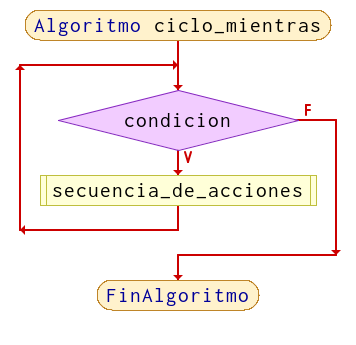
\includegraphics[scale=0.5]{06-while.png}
      \end{center}
    \column{0.5\textwidth}
    \begin{itemize}
      \item Son tambíen conocidas como \textbf{ciclos} o \textbf{bucles}.
      \pausa
      \item Un ciclo es utilizado para ejecutar instrucciones repetidamente.
      \pausa
      \item Python, tiene dos tipos de estructuras repetitivas:
        \begin{itemize}
          \item \textcolor{codeKeyword}{while}
          \item \textcolor{codeKeyword}{for}
        \end{itemize}
    \end{itemize}
  \end{columns}
\end{frame}

\section{El ciclo/bucle "mientras"}

\begin{frame}[fragile]
  \frametitle{Sentencia Mientras}
  Con en ciclo \textbf{mientras} podemos ejecutar un conjunto de
  declaraciones siempre que una condición sea verdadera.

  \begin{columns}
    \column{0.5\textwidth}
    La representación de un ciclo mientras en pseudocódigo.
    \vspace{\baselineskip}
    \begin{lstlisting}[style=pseudocodigo]
Mientras condición_lógica Hacer
		secuencia_de_acciones
Fin Mientras
    \end{lstlisting}

    \column{0.5\textwidth}
    \pausa
    La representación de un ciclo mientras en diagrama de flujo.
    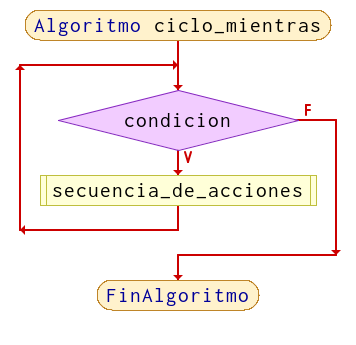
\includegraphics[scale=0.4]{06-while.png}
  \end{columns}
\end{frame}

\begin{frame}[fragile]
  \frametitle{Sentencia Mientras}

  En Python la sentencia del ciclo \textbf{mientras} es
  \textcolor{codeKeyword}{while} y termina con dos puntos ":".

  \vspace{\baselineskip}
  \begin{lstlisting}[language=Python]
  while condicion:
     accion_1
     accion_2
     accion_3
  \end{lstlisting}
\end{frame}

\begin{frame}[fragile]
  \frametitle{Sentencia Mientras}

  Ejemplo: mientras \textbf{contador} sea menor a 6, imprimir el valor
  de \textbf{contador}.

  \vspace{\baselineskip}
  \begin{lstlisting}[language=Python]
  contador = 1
  while contador < 6:
    print(contador)
    contador += 1 # es lo mismo que: contador = contador + 1
  \end{lstlisting}

  \pausa
  \begin{alertblock}{Nota}
    Recuerde incrementar \textbf{i}, de lo contrario el ciclo continuará
    para siempre.
  \end{alertblock}

  El \emph{ciclo while} requiere que las variables relevantes estén listas,
  en este ejemplo necesitamos definir una variable de indexación, contador,
  que establecemos en 1.
\end{frame}

\begin{frame}[fragile]
  \frametitle{Sentencia \textbf{break}}

  Con la sentencia \textcolor{codeKeyword}{break} podemos detener el ciclo incluso si la
  condición while es verdadera:

  \vspace{\baselineskip}
  \begin{lstlisting}[language=Python]
  contador = 1
  while contador < 6:
    print(contador)
    if contador == 3:
      break
    contador += 1
  \end{lstlisting}
\end{frame}

\begin{frame}[fragile]
  \frametitle{Sentencia \textbf{continue}}

  Con la declaración \textcolor{codeKeyword}{continue} podemos detener la iteración actual
  y continuar con la siguiente:

  \vspace{\baselineskip}
  \begin{lstlisting}[language=Python]
  contador = 0
  while contador < 6:
    contador += 1
    if contador == 3:
      continue
    print(contador)
  \end{lstlisting}
\end{frame}

\begin{frame}[fragile]
  \frametitle{Sentencia \textbf{else}}

  Con la instrucción \textcolor{codeKeyword}{else} podemos ejecutar un bloque de código
  una vez cuando la condición ya no es verdadera:

  \vspace{\baselineskip}
  \begin{lstlisting}[language=Python]
  contador = 1
  while contador < 6:
    print(contador)
    contador += 1
  else:
    print("contador ya no es menor que 6")
  \end{lstlisting}
\end{frame}

\section{El ciclo/bucle "para"}

\begin{frame}[c]{El ciclo for}

  Un bucle \textcolor{codeKeyword}{for} se usa para iterar sobre una secuencia
  (que es una lista, una tupla, un diccionario, un conjunto o una cadena).

  \vspace{\baselineskip}
  Esto es menos parecido a la palabra clave \textcolor{codeKeyword}{for} en
  otros lenguajes de programación y funciona más como un método
  \textbf{iterador} que se encuentra en otros lenguajes de programación
  orientados a objetos.
\end{frame}

\begin{frame}[fragile]
  \frametitle{El bucle for}

  Con el ciclo for podemos ejecutar un conjunto de declaraciones,
  una vez para cada elemento de una lista, tupla, conjunto, etc.

  \vspace{\baselineskip}
  \begin{lstlisting}[language=Python]
  frutas = ["manzana", "platano", "cereza"]
  for x in frutas:
    print(x)
  \end{lstlisting}

  \vspace{\baselineskip}
  El bucle for no requiere que se establezca una variable de
  indexación de antemano.
\end{frame}

\begin{frame}[fragile]
  \frametitle{Iterando en una cadena de texto}

  Incluso las cadenas son objetos iterables, contienen una
  secuencia de caracteres:

  \vspace{\baselineskip}
  \begin{lstlisting}[language=Python]
  for x in "manzana":
    print(x)
  \end{lstlisting}
\end{frame}

\begin{frame}[fragile]
  \frametitle{Sentencia \textbf{break}}

  \vspace{\baselineskip}
  Con la instrucción \textcolor{codeKeyword}{break} podemos detener el ciclo
  antes de que haya pasado por todos los elementos:

  \vspace{\baselineskip}
  \begin{lstlisting}[language=Python]
  frutas = ["manzana", "platano", "naranja"]
  for x in frutas:
    print(x)
    if x == "platano":
      break
  \end{lstlisting}

  \pausa
  \begin{lstlisting}[language=Python]
  frutas = ["manzana", "platano", "naranja"]
  for x in frutas:
    if x == "platano":
      break
    print(x)
  \end{lstlisting}
\end{frame}

\begin{frame}[fragile]
  \frametitle{Sentencia \textbf{continue}}

  Con la instrucción \textcolor{codeKeyword}{continue} podemos detener
  la iteración actual del ciclo y continuar con la siguiente:

  \vspace{\baselineskip}
  \begin{lstlisting}[language=Python]
  frutas = ["manzana", "platano", "naranja"]
  for x in frutas:
    if x == "platano":
      continue
    print(x)
  \end{lstlisting}
\end{frame}

\begin{frame}[fragile]
  \frametitle{La función \textbf{range}()}

  Para recorrer un conjunto de código un número de veces específico,
  podemos usar la función \textcolor{codeKeyword2}{range}(),

  \vspace{\baselineskip}
  La función \textcolor{codeKeyword2}{range}() devuelve una secuencia
  de números, comenzando desde \textbf{0} de forma predeterminada,
  se incrementa en 1 (de forma predeterminada) y termina en un
  número especificado.

  \vspace{\baselineskip}
  \begin{lstlisting}[language=Python]
  for x in range(6):
    print(x)
  \end{lstlisting}

  \pausa
  \begin{alertblock}{Nota}
  Tenga en cuenta que la función range(6) no son los valores de 0 a 6,
  sino los valores de 0 a 5.
  \end{alertblock}
\end{frame}

\begin{frame}[fragile]
  \frametitle{La función \textbf{range}()}

  La función \textcolor{codeKeyword2}{range}() tiene por defecto 0
  como valor inicial, sin embargo, es posible especificar el valor
  inicial agregando un parámetro: \textcolor{codeKeyword2}{range}(2, 6),
  que significa valores de 2 a 6 (pero sin incluir 6):

  \vspace{\baselineskip}
  \begin{lstlisting}[language=Python]
  for x in range(2, 6):
    print(x)
  \end{lstlisting}
\end{frame}

\begin{frame}[fragile]
  \frametitle{La función \textbf{range}()}

  La función \textcolor{codeKeyword2}{range}() tiene como valor
  predeterminado incrementar la secuencia en 1, sin embargo, es
  posible especificar el valor de incremento agregando un tercer
  parámetro: \textcolor{codeKeyword2}{range}(2, 30, 3):

  \vspace{\baselineskip}
  \begin{lstlisting}[language=Python]
  for x in range(2, 30, 3):
    print(x)
  \end{lstlisting}
\end{frame}

%\begin{frame}[c]{Pseudocodigo \textbf{para}}
  %\includegraphics[scale=0.3]{12-psc_for.png}
  %\pausa
  %\includegraphics[scale=0.35]{12-df_for.png}
%\end{frame}
\begin{frame}[fragile]
  \frametitle{Pseudocódigo \textbf{para}}
  La representación de un ciclo \textbf{para} en pseudocódigo.
  \begin{lstlisting}[style=pseudocodigo]
Para variable_numerica <- valor_inicial Hasta valor_final Con Paso incremento Hacer
		secuencia_de_acciones
Fin Para
  \end{lstlisting}

  La representación de un ciclo \textbf{para} en diagrama de flujo.
  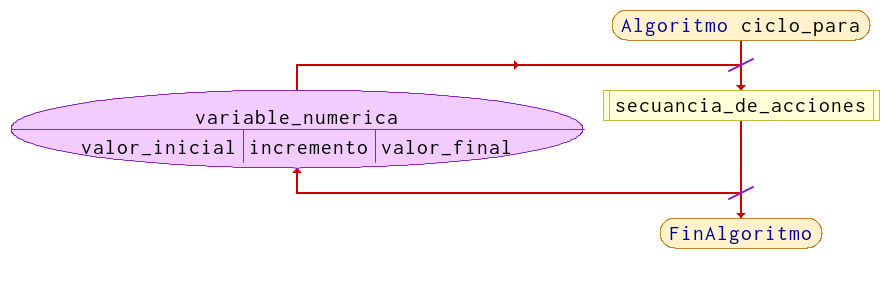
\includegraphics[scale=0.4]{06-for.png}
\end{frame}


\begin{frame}[fragile]
  \frametitle{\textbf{Else} en ciclo \textbf{for}}

  La palabra clave \textcolor{codeKeyword2}{else} en un bucle for
  especifica un bloque de código que se ejecutará cuando
  finalice el bucle:

  \vspace{\baselineskip}
  \begin{lstlisting}[language=Python]
  for x in range(6):
    print(x)
  else:
    print("Al fin termino!")
  \end{lstlisting}
\end{frame}

\begin{frame}[fragile]
  \frametitle{\textbf{Else} en ciclo \textbf{for}}

  \begin{alertblock}{Nota}
    El bloque else NO se ejecutará si el bucle se detiene
    mediante una declaración de interrupción (break).
  \end{alertblock}

  \vspace{\baselineskip}
  \begin{lstlisting}[language=Python]
  for x in range(6):
    if x == 3: break
    print(x)
  else:
    print("Al fin termino!")
  \end{lstlisting}
\end{frame}

\begin{frame}[fragile]
  \frametitle{Ciclos anidados}

  Un bucle/ciclo anidado es un bucle/ciclo dentro de un bucle/ciclo.

  \vspace{\baselineskip}
  El "bucle interno" se ejecutará una vez por cada iteración del
  "bucle externo":

  \vspace{\baselineskip}
  \begin{lstlisting}[language=Python]
  adjetivo = ["roja", "grande", "dulce"]
  frutas = ["manzana", "platano", "naranja"]

  for x in adjetivo:
    for y in frutas:
      print(y, x)
  \end{lstlisting}
\end{frame}

\begin{frame}[fragile]
  \frametitle{La sentencia \textbf{pass}}

  Los bucles for no pueden estar vacíos, pero si por alguna
  razón tiene un bucle for sin contenido, ingrese la instrucción
  pass para evitar errores.

  \vspace{\baselineskip}
  \begin{lstlisting}[language=Python]
  for x in [0, 1, 2]:
    pass
  \end{lstlisting}
\end{frame}
